\documentclass[]{article}

\usepackage{graphicx}

%opening
\title{Figures for  3-D printed oxygen devices}
\author{}

\begin{document}

%\maketitle

\section{figures}

\begin{figure}[H]
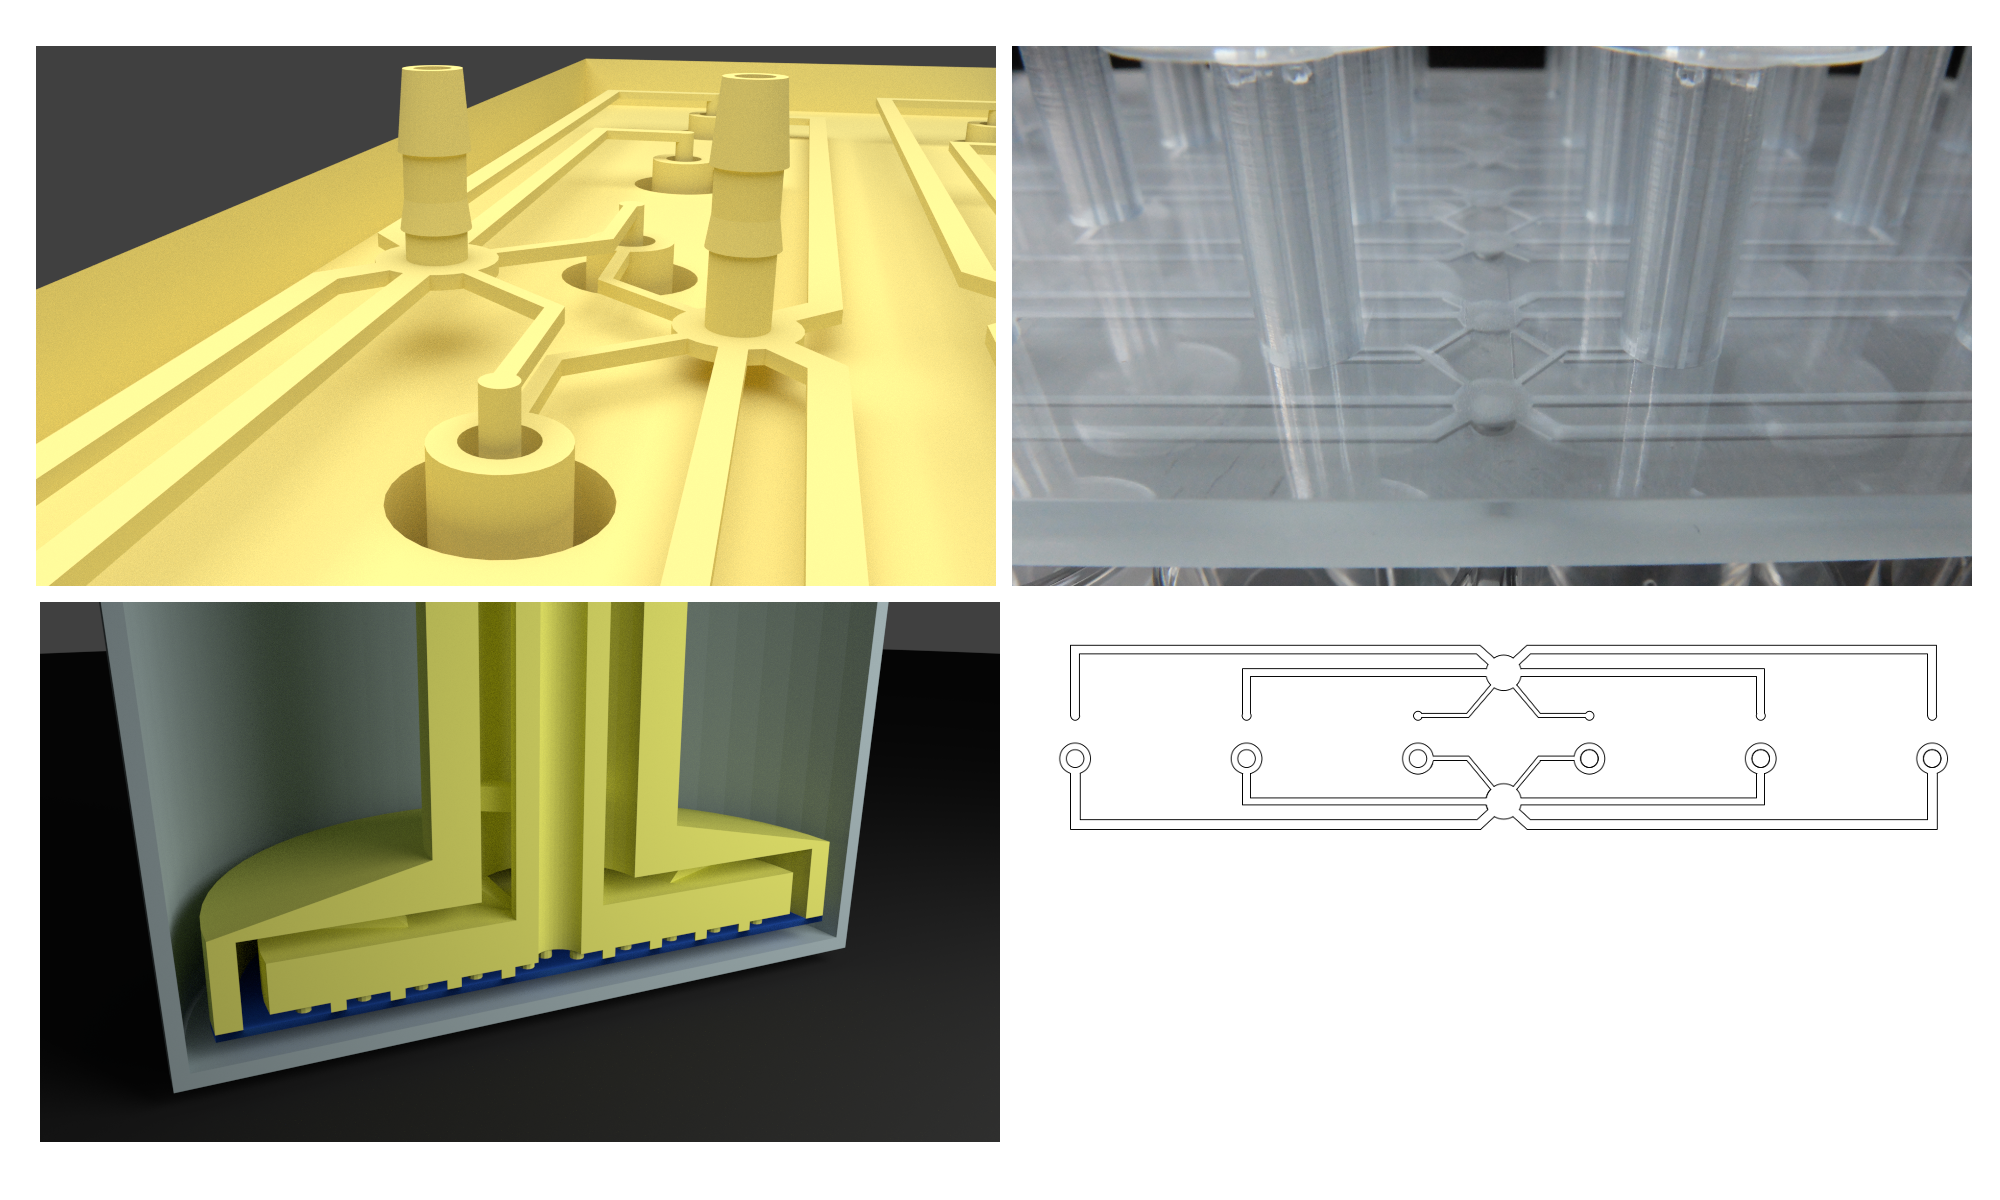
\includegraphics[scale=.75]{fig1.png} 
\caption{
{\bf Design of 24-well Insert Device.}
(A) Rendering of whole 3D printed part.
An inlet and outlet barb allows perfusion of gas to control 6 channels.
(B) At the bottom of each pillar gas entering from the outer channel flows along the PDMS membrane (blue), which is supported by micropillars, and exhausts via the inner pipe.
Diffusion occurs rapidly through the PDMS membrane to the cell culture spaced 500 $\mu$m away at the bottom of the well.
(C) Cross-section demonstrating how the microfluidic distribution network and double pipes are connected. 
The two adjacent mirrored distribution networks are spaced 1 mm apart along the z-axis allowing them to overlap and enter the separate vertical pipes.
The arrows indicate the flow direction.
The incoming gas enters enters the outer pipe on its way to the bottom of the well and returns through the inner pipe.
(D) Photo of the device with dyed channels in a 24-well plate.
(E) Photo of the device from the bottom with four independent channel networks.
(F) Photo of the printed distrubution networks.
}
\label{figure1}
\end{figure}

\begin{figure}[H]
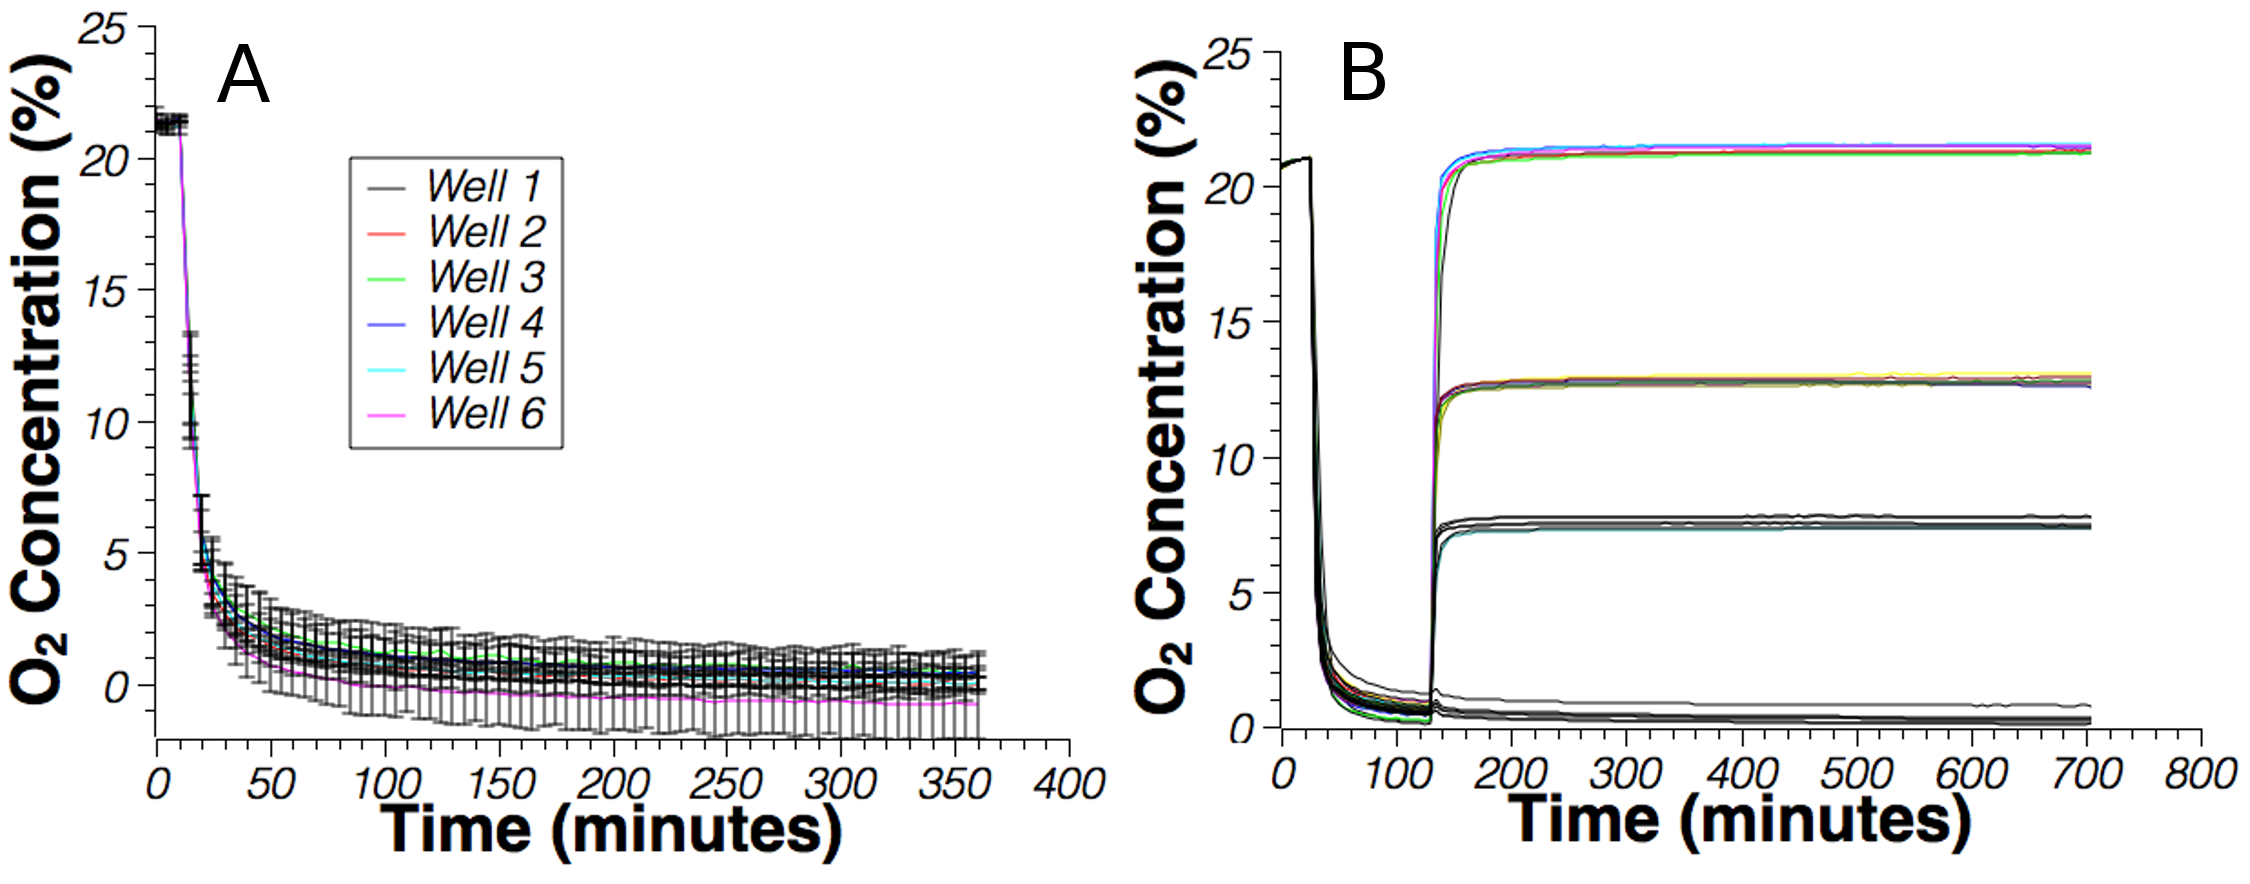
\includegraphics[scale=0.15]{fig2.png}
\caption{
{\bf Oxygen Characterization.} 
(A) Time course data of oxygen being evacuated from the culture area as 0\% oxygen gas is perfused through the device.
Error bars are the standard deviation N=3.
(B) Four oxygen conditions are demonstrated in a 24-well plate.
Each 6-well row of the plate can be controlled independently.  
Mean N=3 error bars not included.
}
\label{figure2}
\end{figure}

\begin{figure}[H]
%\includegraphics[scale=0.2]{image.jpg} % remove for manuscript submission
\caption{
{\bf PCR Data.}  Not finished yet.  
}
\label{pcr-data}
\end{figure}

%\begin{abstract}

%\end{abstract}

%\section{}

\end{document}
